\documentclass[10pt]{article}
\usepackage{amsmath} % assumes amsmath package installed
\usepackage{amsfonts,mathrsfs}
\usepackage{amssymb}
\usepackage{color}
\usepackage{graphicx}
\usepackage{epsfig}
\usepackage{epstopdf}
\usepackage{subfigure}
\usepackage{enumerate}
\usepackage{algorithm,algorithmicx}
\usepackage{algpseudocode}

%\usepackage[]{algorithm2e}

\def\bbbr{{\rm I\!R}}
%\input{macros.tex}
%\input{slide_macros.tex}

\newtheorem{definitiox	n}{Definition}{\it}{}
\newtheorem{example}{Example}{\it}{}
\newtheorem{corollary}{Corollary}{\it}{}
\newtheorem{proposition}{Proposition}{\it}{}
\newtheorem{lemma}{Lemma}{\it}{}
\newtheorem{theorem}{Theorem}{\it}{}
\newtheorem{remark}{Remark}{\it}{}
\newtheorem{assumption}{Assumption}{\it}{}
\newenvironment{proof}[1][Proof]{\noindent\textbf{#1.} }{\ \rule{0.5em}{0.5em}}
%\newcommand{\proof}{\vspace{1mm}\noindent{\it Proof.}\quad}
%\def\qed{\quad{$\square$}} 

\textwidth=6.3in
\textheight 9in 
\setlength{\topmargin}{-0.5in}
\setlength{\oddsidemargin}{0.1in} 
\setlength{\evensidemargin}{0.1in}
%%%%%%%%%%%%%%%%%%%%%%%%%%%%%%%%%%
\def\an#1{{{\bf \color{blue}#1}}}
\def\o{\omega}
\def\vmean{v^{\rm mean}}
\def\vmax{v^{\rm max}}	
\def\e{\epsilon}
\newcommand{\todo}[1]{\vspace{5 mm}\par \noindent \marginpar{\textsc{ToDo}}
\framebox{\begin{minipage}[c]{0.9 \textwidth} \tt #1
\end{minipage}}\vspace{5 mm}\par}

% Boldsymbols, mathcal, mathbb
\newcommand{\bs}{\boldsymbol}
\newcommand{\mc}{\mathcal}
\newcommand{\bb}{\mathbb}
\newcommand{\R}{\bb R}

%norm
\newcommand{\norm}[1]{\left\|#1\right\|}

% Operators and notations
\newcommand{\dom}{\operatorname{dom}}
\newcommand{\iP}{\mathcal{P}}
\newcommand{\B}{\mathcal{C}}
\newcommand{\red}{\textcolor{red}}
\newcommand{\blue}{\textcolor{blue}}
\newcommand{\argmin}{\operatorname{argmin}}
\newcommand{\mini}{\operatorname{minimize}}
\newcommand{\Proj}{\mathrm{Proj}}
\newcommand{\fix}{\mathrm{fix}}
\newcommand{\proj}{\mathrm{proj}}
\newcommand{\prox}{\mathrm{prox}}
\newcommand{\Id}{\mathrm{Id}}
\newcommand{\Res}{\operatorname{J}}
\newcommand{\diag}{\operatorname{diag}}
\newcommand{\blkdiag}{\operatorname{blkdiag}}
\newcommand{\col}{\operatorname{col}}
\newcommand{\zer}{\operatorname{zer}}
\newcommand{\nulls}{\operatorname{Null}}
\newcommand{\range}{\operatorname{Range}}
\newcommand{\dist}{\mathrm{dist}}
\newcommand{\nc}{\mathrm{N}}
\newcommand{\0}{\mathbf{0}}
\newcommand{\1}{\mathbf{1}}
\newcommand{\half}{^1\hspace*{-.1em}/_2}

%Roman numbers
\newcommand{\rmnum}[1]{\romannumeral #1}
\newcommand{\Rmnum}[1]{\expandafter\@slowromancap\romannumeral #1@}


%%%%%%%%%%%%%%%%%%%%%%%%%%%%%%%%%%%%%%%

\title{Decentralized Algorithms for Generalized Nash Equilibrium Seeking in Peer-to-peer Electricity Markets}
\author{Giuseppe Belgioioso}
\begin{document}
\maketitle

%%%%%%%%%%%%%%%%%%%%%%%%%%%%%%%%%%%%%
\section{Problem statement}
Consider the same problem statement in \texttt{problem\_setup\_v7.tex}.

%%%%%%%%%%%%%%%%%%%%%%%%%%%%%%%%%%%%%%%%%%%%%%%%%%%%%%

\section{Algorithms}
\subsection{Semi-decentralized}

The algorithm presented in this section corresponds to \cite[Alg. 6B]{belgioioso2020semi} applied on  \texttt{problem\_setup\_v6.tex}.

Consider the following choices for the step-sizes in Algorithm 1.
\smallskip

\begin{assumption}[Step-size]\label{ass:SSS}
Set the step sizes of prosumers and DSO as follows:
\begin{enumerate}[(i)]
\item $\forall i \in \mc N$: set $A_i = \diag( \alpha_{i}^{\text{pi}}, \alpha_{i}^{\text{st}} , \alpha_{i}^{\text{mg}} , \{ \alpha_{(i,j)}^{\text{tr}} \}_{j \in \mc N_i} ) \otimes I_H$, with $\alpha_{i}^{\text{pi}}, \alpha_{i}^{\text{st}} > 1$, $ \alpha_{i}^{\text{mg}} > 3 + N \max_{h\in \mc H} d_h^{\text{mg}} $, $\alpha_{(i,j)}^{\text{tr}} > 2$, $\forall j \in \mc N_i$, $\beta^{\text{tr}}_{(i,j)} = \beta^{\text{tr}}_{ (j,i)} < \frac{1}{2}$, $\forall j \in \mc N_i$. 

\item Set $A_{N+1}:=\diag\left(
\left\{
\alpha_y^{\theta},\alpha^{\text v}_y, \alpha_y^{\text{tg}},
\{ 
\alpha^\text{p}_{(y,z)}, \alpha^{\text{q}}_{(y,z)} 
\}_{z \in \mc B_y}
\right\}_{y \in \mc B}
\right) \otimes I_H
$, with $\alpha_y^{\theta},\alpha^{\text v}_y > 0$, $\alpha_y^{\text{tg}} > 2$, $\alpha^{\text{p}}_{(y,z)} > 1$ and $ \alpha^{\text{q}}_{(y,z)} > 0 $, $\forall z \in \mc B_y$, $ \forall y \in \mc B$.
Set $\gamma^{\text{mg}} < \frac{1}{N}$, $\beta^{\text{tg}} < (|\mc N| + |\mc B|)^{-1}$ and $\beta_y^{\text{pb}} < (1+2|\mc N_y|+|\mc B_y|)^{-1}$, for all $y \in \mc B$.
{\hfill $\square$}
\end{enumerate}


\end{assumption}




\newpage
%%%%%%%%

\algblockdefx[DSO]{DSO}{EndDSO}
[1][<default value>]{\textbf{DSO update}}
[2][<default value>]{\textbf{end}}

\algblockdefx[PRO]{PRO}{EndPRO}
[1][<default value>]{\textbf{Prosumer $i$ update}}
[2][<default value>]{\textbf{end prosumer $i$ update}}

\algblockdefx[Primal]{Primal}{EndPrimal}
[1][<default value>]{\textbf{primal update}}
[2][<default value>]{\textbf{end}}

\algblockdefx[Dual]{Dual}{EndDual}
[1][<default value>]{\textbf{dual update}}
[2][<default value>]{\textbf{end}}

\algblockdefx[Aux]{Aux}{EndAux}
[1][<default value>]{\textbf{auxiliary update}}
[2][<default value>]{\textbf{end}}

\algblockdefx[Comm]{Comm}{EndComm}
[1][<default value>]{\textbf{communication}}
[2][<default value>]{\textbf{end}}

\algblockdefx[Agg]{Agg}{EndAgg}
[1][<default value>]{\textbf{aggregation update}}
[2][<default value>]{\textbf{end}}

\algblockdefx[IUC]{IUC}{EndIUC}
[1][<default value>]{\textbf{Iterate until convergence}}
[2][<default value>]{\textbf{end}}
%%%%%%%%%%

\begin{algorithm}[H]
\caption{Semi-decentralized GWE seeking for P2P Energy Markets}
\begin{algorithmic}[1]
	%
%\Procedure{Initialization prosumers}{}
%\ForAll{prosumer $ i \in \mc N$}
%\State  Set the initial conditions: $u_i(0) \in \mc U_i$, $\mu^{\text{tr}}_{(i,j)}(0) = \0$, $\forall j \in \mc N_i$.
%\State  Set the step sizes as in Assumption \ref{ass:SSS}(i).
%\EndFor
%\EndProcedure
%\Procedure{Initialization DSO}{}
%\State  Set the initial conditions: $u_{N+1}(0) \in \mc U_{N+1}$, $\lambda^{\text{mg}}=\0$, $\mu^{\text{tg}} = \0$, $\mu_y^{\text{pb}}(0) = \0$, $\forall y \in \mc B$.
%\State Set the step sizes as in Assumption \ref{ass:SSS}(ii).
%\EndProcedure
\medskip
\IUC{ }


\ForAll{prosumer $ i \in \mc N$}
\Primal{ }
\Comment{power generated, stored, from the grid, traded}

\smallskip
\State 
$a_i(k) = 
	\col \big(-\mu_y^{\text{pb}}(k),-\mu_y^{\text{pb}}(k),
	{
	%\left(
	\left[
	\begin{smallmatrix}
	I_H\\
	- I_H 
	\end{smallmatrix}
	\right] 
	%\otimes I_H
%\right)	
	}^\top \lambda^{\text{mg}}(k) + \mu^{\text{tg}}(k),
	%
	\left\{ {\mu^{\text{tr}}_{(i,j)}(k)}\right\}_{j \in \mc N_i}   \big)$
\Comment{aux. vector}

\State
$u_i(k+1)   =
\left\{
\begin{array}{r l}
	\underset{\xi \in \R^{n_i}}{\argmin} & 
	J_{i} \big( \xi, \sigma^{\text{mg}}(k) \big) 
	+ {a_i(k)}^\top \xi + \frac{1}{2}
	\left\| \xi - u_i(k) 
	\textstyle
	  \right\|^2_{A_i} \\
	\text{s.t. } & \xi \in \mc U_i
\end{array} 
	\right.	$
\Comment{quadratic progr.}	
\EndPrimal

\Comm{ }
\Comment{to DSO and trading partners}
\State $b_i(k+1)= p^{\text{d}}_i-p^{\text{di}}_i(k+1)- p^{\text{st}}_i(k+1)$
\Comment{local load unbalance of prosumer $i$}
\State
$
p^{\textrm{mg}}_{i}(k+1), b_i(k+1)  \longrightarrow  \text{DSO,}
$
\Comment{forward to DSO}
     \ForAll{prosumer $ j \in \mc N_i$}
     
\State
 $p^{\text{tr}}_{(i,j)}(k+1)
	\longrightarrow \text{prosumer }j$
	\Comment{forward local trade to prosumer $j$}
	\EndFor
\EndComm


\Dual{ }
\Comment{reciprocity constraints}
\ForAll{$ j \in \mc N_i$}
\State
$c^{\text{tr}}_{(i,j)}(k+1)  =  p^{\textrm{tr}}_{(i,j)} (k+1) + p^{\textrm{tr}}_{(j,i)} (k+1)$
\Comment{aux. vector}
\State
$\mu^{\text{tr}}_{(i,j)}(k+1) = \mu_{(i,j)}(k) + \beta_{ij}^{\text{tr}} \left( 
	2  c^{\text{tr}}_{(i,j)}(k+1) - c^{\text{tr}}_{(i,j)}(k)
	\right)$
	\Comment{reflected dual ascent}
\EndFor

\EndDual

\EndFor

%%%%%%%%%%%%%%%%%%%%%%
%\Statex
\DSO{ }

\Primal{}
\Comment{physical variables}
\State
$a_{N+1}(k) = \col \left( 
	\left\{
	\0,\0,-\mu^{\text{tg}}(k) - \mu_y^{\text{pb}}(k), 
	\{ -\mu_y^{\text{pb}}(k), \0 \}_{z \in \mc B_y}
	\right\}_{y \in \mc B}
	\right)$
\Comment{aux. vector}

\State 	$u_{N+1}(k+1) = \proj_{\mc U_{N+1}}  \left( u_{N+1}(k) - A_{N+1} a_{N+1}(k) \right)$
\Comment{ solved via Algorithm 2 }
\EndPrimal

%---------------------------Aggregation
\Agg{}
\State
$ \sigma^{\text{mg}}(k+1) = \sum_{i \in \mc N} p_i^{\text{mg}}(k+1) $
\Comment{aggregate grid-to-prosumers power }
\State
$\sigma^{\text{tg}}(k+1) = \sum_{y \in \mc B} p_y^{\text{tg}}(k+1)$
\Comment{aggregate grid-to-buses power }
\EndAgg

%---------------------------Dual Update
\Dual{}
\State
$b_{N+1}(k+1	) = 
	\left[
	\begin{smallmatrix}
	1\\
	- 1 
	\end{smallmatrix}
	\right] \otimes (2 \sigma^{\text{mg}}(k+1)- \sigma^{\text{mg}}(k)) 
	-
	\left[
	\begin{smallmatrix}
	\overline{p}^{\mathrm{mg}}\1_{H} \\
	-     \underline{p}^{\mathrm{mg}} \1_{H}
	\end{smallmatrix} 
	\right]  $
	\Comment{aux. vector}
	\State
$\lambda^{\text{mg}}(k+1) = \textstyle
	\proj_{\R^{2 H}_{\geq 0}}\left( 
	\lambda^{\text{mg}}(k) + \gamma^{\text{mg}} b_{N+1}(k+1)
	 \right)$
		\Comment{grid constraints}

\ForAll{buses $ y \in \mc B$}

\State
$c^{\text{pb}}_y(k+1)   = p_y^{\text{pd}} + \sum_{i \in \mc N_y} b_i(k+1)- p^{\text{tg}}_y(k+1) - \sum_{z \in \mc B_y} p^\ell_{(y,z)} (k+1)$
\Comment{aux. vector}

\State
$\mu_y^{\text{pb}}(k+1) = \mu_y^{\text{pb}}(k) + \beta^{\text{pb}}_y (2 c^{\text{pb}}_y(k+1)- c^{\text{pb}}_y(k))$
\Comment{local power balance of bus $y$}
\EndFor

\State
$c^{\text{tg}}(k+1) = \sigma^{\text{mg}}
	(k+1)- \sigma^{\text{tg}}(k+1)$
\Comment{aux. vector}

\State
$\mu^{\text{tg}}(k+1) = \mu^{\text{tg}}(k) + \beta^{\text{tg}} (2c^{\text{tg}}(k+1)-c^{\text{tg}}(k))$
\Comment{grid-to-buses constraints}
\EndDual	

\Comm{ }
\Comment{broadcast}
\State
$ \{ \sigma(k+1), \, \lambda^{\text{mg}}(k+1), \mu^{\text{tg}}(k+1) \} 
	\longrightarrow  \mc N$
\Comment{to all prosumers}
\ForAll{buses $ y \in \mc B$}
\State
$\mu^{\text{pb}}_y(k+1)\longrightarrow \mc N_y$
\Comment{to all prosumers on bus $y$}
\EndFor

\EndComm

\EndDSO	

\EndIUC	

\end{algorithmic}
\end{algorithm}

\begin{figure}
\centering
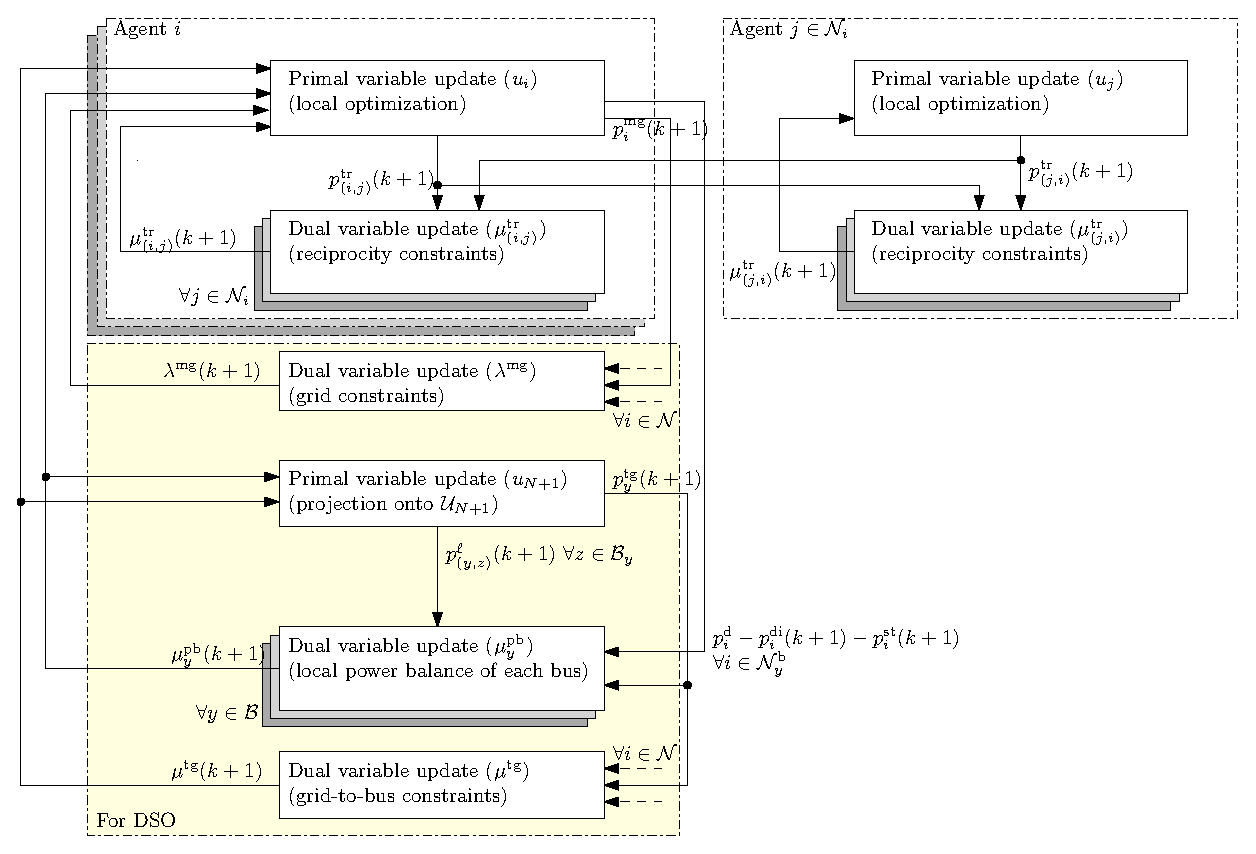
\includegraphics[scale=0.8]{Algorithm1_v2.eps}
\caption{Flowchart of the iterations in Algorithm 1 for agent $i \in \mc N$ and DSO. It also shows the flow of information between agent $i$ and DSO as well as between agent $i$ and its trading partner $j$.}
\end{figure}

%%%%%%%%%%%%%%%%%%%%%%%%%%%%%%%%%%%%%%%%%%%

\subsection{Projection onto $\mc U_{N+1}$}
Next, we propose an iterative method to solve line 24 in Algorithm 1, namely, to compute the projection onto $\mathcal{U}_{N+1}$. First, let us define the sets $C_1 := (17)\cap(18)\cap(19)\cap(20) $ and $C_2 = (15)\cap(16)$ and recall that the decision vector of the DSO reads as $u_{N+1}=\col\left(\{\theta_y, v_y, p_y^{\mathrm{tg}},\{p_{(y,z)}^{\ell},q_{(y,z)}^{\ell}\}_{z \in \mc B_y} \}_{y\in\mc B} \right)$. The projection onto $C_1$ can be characterize in closed-form as follows:
\begin{align*}
\proj_{C_1}(u_{N+1})=
\col\left(\{\theta_y^+, v_y^+, {p_y^{\mathrm{tg}}}^+,\{ {p_{(y,z)}^{\ell}}^+, {q_{(y,z)}^{\ell}}^+ \}_{z \in \mc B_y} \}_{y\in\mc B} \right),
\end{align*}
where, for all $y \in \mc B$,
\begin{align*}
\theta_y^+ &=
\begin{cases}
\underline{\theta}_y, & \text{if } \theta_y < \underline{\theta}_y\\
\overline{\theta}_y, & \text{if } \theta_y > \overline{\theta}_y\\
\theta_y, & \text{otherwise } \
\end{cases}, &  \\
%
v_y^+ &= 
\begin{cases}
\underline{v}_y, & \text{if } v_y < \underline{v}_y\\
\overline{v}_y, & \text{if } v_y > \overline{v}_y\\
v_y, & \text{otherwise } \
\end{cases}
 & \\
%
{p_y^{\text{tg}}}^+ &= 
\begin{cases}
p_y^{\text{tg}}, & \text{if } y \in \mc B^{\text{mg}}\\
0, & \text{otherwise} 
\end{cases}
\\
%
{(p^\ell_{(y,z),h})}^+ & = \frac{\overline{s}_{(y,z)}}{
\max \left\{ \|\col(p^\ell_{(y,z),h)} , q^\ell_{(y,z),h)} \|, \overline{s}_{(y,z)} \right\}
} p^\ell_{(y,z),h},& \quad \forall z \in \mc B_y, \forall h \in \mc H \\
{(q^\ell_{(y,z),h})}^+ & = \frac{\overline{s}_{(y,z)}}{
\max \left\{ \|\col(p^\ell_{(y,z),h)} , q^\ell_{(y,z),h)} \|, \overline{s}_{(y,z)} \right\}
} q^\ell_{(y,z),h} , & \quad \forall z \in \mc B_y, \forall h \in \mc H
\end{align*}
The projection onto $C_2$ can be computed by solving a quadratic programming (e.g. via lsqlin, quadprog, osqp, etc...) with appropriate matrices.

\begin{algorithm}[]
\caption{Douglas--Rachford splitting to compute the projection of $x$ onto $\mathcal{U}_{N+1} = C_1 \cap C_2$}
\begin{algorithmic}[1]

\smallskip
\IUC{ }

\smallskip
\State
$z(k) = \proj_{C_1}(\frac{1}{2} \xi(k) + \frac{1}{2}x)$ 


\smallskip
\State
$\xi(k+1) = \xi(k) + \lambda \left( \proj_{C_2}    (2z(k)-\xi(k)) - z(k)
\right), \quad \text{ with } \lambda \in (0,2)
$
\EndIUC

\end{algorithmic}
\end{algorithm}

\newpage

%%%%%%%%%%%%%%%%%%%%%%%%%%%%%%%%%%%%%%%%%%%%%%%%
\newpage
\subsection{Fully-distributed}



Consider the following choices for the step-sizes.
\begin{assumption}[Step size selection]\label{ass:FD-SSS}
Set the step sizes of prosumers and DSO as follows:
\begin{enumerate}[(i)]
\item $\forall i \in \mc N$: set $A_i = \diag( \alpha_{i}^{\text{pi}}, \alpha_{i}^{\text{st}} , \alpha_{i}^{\text{mg}} , \{ \alpha_{(i,j)}^{\text{tr}} \}_{j \in \mc N_i} ) \otimes I_H$, with $\alpha_{i}^{\text{pi}}, \alpha_{i}^{\text{st}} > 1$, $ \alpha_{i}^{\text{mg}} > 3 + N \max_{h\in \mc H} d_h^{\text{mg}} $, $\alpha_{(i,j)}^{\text{tr}} > 2$, $\forall j \in \mc N_i$, $\beta^{\text{tr}}_{(i,j)} = \beta^{\text{tr}}_{ (j,i)} < \frac{1}{2}$, $\forall j \in \mc N_i$. 

\item $\forall y \in \mc B$: set $A_{y}:=\diag\left(
\alpha_y^{\theta},\alpha^{\text v}_y, \alpha_y^{\text{tg}},
\{ 
\alpha^\text{p}_{(y,z)}, \alpha^{\text{q}}_{(y,z)} 
\}_{z \in \mc B_y}
\right) \otimes I_H
$, with $\alpha_y^{\theta},\alpha^{\text v}_y > 2|\mc B_y |(\|B\|+\|G\|)$, $\alpha_y^{\text{tg}} > 2$, $\alpha^{\text{p}}_{(y,z)} > 2$ and $ \alpha^{\text{q}}_{(y,z)} > 1 $, $\forall z \in \mc B_y$, $ \forall y \in \mc B$. Set $\delta^{\text{mg}}_y = \delta^{\text{mg}} <\frac{1}{2}$, $\delta^{\text{tg}}_y = \delta^{\text{tg}} <\frac{1}{2}$. Set $\gamma^{\text{mg}}_y < (|\mc N_y| + |\mc B_y|)^{-1}$. Set $\beta^{\text{tg}}_y < ( 2|\mc N_y| + |\mc B_y|)^{-1}$ and $\beta_y^{\text{pb}} < (1+2|\mc N_y|+|\mc B_y|)^{-1}$.
Set $\beta^{p,c}_{(z,y)} = \beta^{p}_{ (y,z)} < (2\|B_{(y,z)}\|+2\|G_{(y,z)}\| + 2)^{-1}$, $\beta^{q,c}_{(z,y)} = \beta^{q}_{(y,z)} < ( 2\|B_{(y,z)}\|+ 2\|G_{(y,z)}\| + 2)^{-1}$, $\forall z \in \mc B_y$. Set $\beta^{p,c}_{(z,y)} = \beta^{p,c}_{ (y,z)} < \frac{1}{2}$, $\beta^{q,c}_{(z,y)} = \beta^{q,c}_{ (y,z)} < \frac{1}{2}$, $\forall z \in \mc B_y$.

{\hfill $\square$}
\end{enumerate}
\end{assumption}

\begin{itemize}
\item the decision variable of bus $y$ is $u_y := \left(
\theta_y, v^{\text v}_y, p_y^{\text{tg}},
\{ 
p^\ell_{(y,z)}, q^{\ell}_{(y,z)} 
\}_{z \in \mc B_y}
\right) \in \mathbb R^{d}$, with $d:= (3+2 |\mc B_y| )24$.

\item
Let us introduce the local sets of constraints of bus $y$, i.e.,
$\mc U_y := \left\{
u \in \R^d \, | \, (17)-(20) \text{ are satisfied}
\right\}.
$

\item We recast the power flow equation (15) as
\begin{align*}
0 &= 2B(\theta_y-\theta_z) - 2G( v_y - v_z) - (p^{\ell}_{(y,z)} - p^{\ell}_{(z,y)})\\
0 &= p^\ell_{(y,z)} + p^\ell_{(z,y)}
\end{align*}

\item Similarly, we recast the power flow equation (16) as
\begin{align*}
0 &= 2G(\theta_y-\theta_z) + 2B( v_y - v_z) - (q^{\ell}_{(y,z)} - q^{\ell}_{(z,y)})\\
0 &= q^\ell_{(y,z)} + q^\ell_{(z,y)}
\end{align*}

\blue{GB:
It is convenient for deriving an effective distributed algorithm. Intuitively, the dual variables of such constraints will evolve (almost) identically on bus $y$ and $z$.
}
\end{itemize}





\begin{algorithm}[H]
\caption{Fully-decentralized GWE seeking for P2P Energy Markets}
\begin{algorithmic}[1]
\Statex
\medskip
\IUC{ }

%------------------For each community/bus y
\ForAll{Bus $ y \in \mc B$ (in parallel)}

\ForAll{prosumer $ i \in \mc N_y$ (in parallel)}
\PRO{}
   \State 
   \textbf{primal update}
   \Comment{power generated, stored, from the grid, traded}

   \State 
   \textbf{communication}
   \Comment{with bus $y$ operator and trading partners $j \in \mc N_i$}

   \State 
   \textbf{dual update}
   \Comment{reciprocity constraints}
\EndPRO      

\EndFor

\DSO{ (local bus $y$ unit)}
\State
\textbf{primal update}
\Comment{local physical variables of bus $y$}
\State
\textbf{aggregation update}
\Comment{ total grid-to-pros. power and load unbalance on bus $y$}
\State
\textbf{auxiliary update}
\Comment{ for consensus of the dual variables}
\State
\textbf{dual update}
\Comment{physical constraints}
\State
\textbf{communication}
\Comment{with prosumers on bus $y$ and neighbouring buses $j \in \mc B_y$}
\EndDSO


\EndFor


\EndIUC	

\end{algorithmic}
\end{algorithm}

%%%%%%%%%%%%%%%%%%%%%%%%%%%%%%%%% Prosumer $i$ update
\begin{algorithm}[H]
\caption{Prosumer $i$ update}
\begin{algorithmic}[1]
\Statex
\Primal{ }
\Comment{power generated, stored, from the grid, traded}
\smallskip
\State 
$a_i(k) = 
	\col \big(-\mu_y^{\text{pb}}(k),-\mu_y^{\text{pb}}(k),
\bar \lambda_y^{\text{mg}}(k) + \mu_y	^{\text{tg}}(k),
	%
	\left\{ {\mu^{\text{tr}}_{(i,j)}(k)}\right\}_{j \in \mc N_i}   \big)$
\Comment{aux. vector}

\State
$u_i(k+1)   =
\left\{
\begin{array}{r l}
	\underset{\xi \in \R^{n_i}}{\argmin} & 
	J_{i} \big( \xi,\sum_{y \in \mc B} \sigma_y^{\text{mg}}(k) \big) 
	+ {a_i(k)}^\top \xi + \frac{1}{2}
	\left\| \xi - u_i(k) 
	\textstyle
	  \right\|^2_{A_i} \\
	\text{s.t. } & \xi \in \mc U_i
\end{array} 
	\right.	$
\Comment{quadratic progr.}	
\EndPrimal

\Comm{ }
%\Comment{to Bus $y$ and trading partners}
\State $b_i(k+1)= p^{\text{d}}_i-p^{\text{di}}_i(k+1)- p^{\text{st}}_i(k+1)$
\Comment{local load unbalance of prosumer $i$}
\State
$
p^{\textrm{mg}}_{i}(k+1), b_i(k+1)  \longrightarrow  \text{Bus y,}
$
\Comment{forward to Bus $y$}
     \ForAll{prosumer $ j \in \mc N_i$}
     
\State
 $p^{\text{tr}}_{(i,j)}(k+1)
	\longrightarrow \text{prosumer }j$
	\Comment{forward local trade to prosumer $j$}
	\EndFor
\EndComm


\Dual{ }
\Comment{reciprocity constraints}
\ForAll{$ j \in \mc N_i$}
\State
$c^{\text{tr}}_{(i,j)}(k+1)  =  p^{\textrm{tr}}_{(i,j)} (k+1) + p^{\textrm{tr}}_{(j,i)} (k+1)$
\Comment{aux. vector}
\State
$\mu_{(i,j)}^{\text{tr}}(k+1) = \mu_{(i,j)}(k) + \beta_{ij}^{\text{tr}} \left( 
	2  c^{\text{tr}}_{(i,j)}(k+1) - c^{\text{tr}}_{(i,j)}(k)
	\right)$
	\Comment{reflected dual ascent}
\EndFor

\EndDual



\end{algorithmic}
\end{algorithm}

%%%%%%%%%%%%%%%%%%%%%%%%%%%%%%%%% End of Prosumer $i$ update
%%%%%%%%%%%%%%%%%%%%%%%%%%%%%%%%% Bus y update

\begin{algorithm}[H]
\caption{DSO bus $y$ update}
\begin{algorithmic}[1]
\Statex
\Primal{}
\Comment{physical variables}
\State
$
a^\theta_{y}(k) = 	
4	\sum_{z\in \mc B_y} \big( B_{(y,z)}^\top  \mu^p_{(y,z)}(k) + G_{(y,z)}^\top \mu^q_{(y,z)}(k) \big)$
\Comment{aux. vector}

\State
$
a^{\text{v}}_{y}(k) = 4	
	\sum_{z\in \mc B_y} \big( B_{(y,z)}^\top  \mu^q_{(y,z)}(k)  - G_{(y,z)}^\top \mu^p_{(y,z) }  (k) \big)$
\Comment{aux. vector}



\State
$
a_{y}(k) = \col \left( 	
	a^\theta_{y}(k),a^{\text{v}}_{y}(k),-\mu_y^{\text{tg}}(k) - \mu_y^{\text{pb}}(k), 
	\left\{ \mu^{p,c}_{(y,z)}(k) -\mu_y^{\text{pb}}(k) - \mu_{(y,z)}^p(k) ,  \mu^{q,c}_{(y,z)} -\mu_{(y,z)}^q(k) \right\}_{z \in \mc B_y}
	\right)$
%\Comment{aux. vector}

\State 	$u_{y}(k+1) = \proj_{\mc U_{y}}  \left( u_{y}(k) - A_{y} a_{y}(k) \right)$
\Comment{ solved via Algorithm 2 }
\EndPrimal

%---------------------------Aggregation
\Agg{}
\State
$ \sigma_y^{\text{mg}}(k+1) = \sum_{i \in \mc N_y} p_i^{\text{mg}}(k+1) $
\Comment{aggregate grid-to-prosumers power on bus $y$}
\State
$b_y(k+1) = \sum_{i \in \mc N_y} b_i(k+1)$
\Comment{aggregate load unbalance on bus $y$ }
\EndAgg


%---------------------------Auxiliary update
\Aux{}
\State
$ w_y^{\text{mg}}(k+1) = w_y^{\text{mg}}(k) + \delta^{\text{mg}}_y \left( |\mc N_y | \lambda^{\text{mg}}_y (k) - \sum_{z \in \mc B_y} \lambda^{\text{mg}}_y (z) \right) $
\Comment{consensus on $\lambda^{\text{mg}}_y$'s}

\State
$ w_y^{\text{tg}}(k+1) = w_y^{\text{tg}}(k) + \delta^{\text{tg}}_y \left( |\mc N_y | \lambda^{\text{tg}}_y (k) - \sum_{z \in \mc B_y} \lambda^{\text{tg}}_y (z) \right) $
\Comment{consensus on $\lambda^{\text{tg}}_y$'s}

\EndAux
\State

%---------------------------Dual Update


\Dual{(global grid constraints)}
\State
$c^{\text{mg}}_{y}(k+1) = 
	\left[
	\begin{smallmatrix}
	1\\
	- 1 
	\end{smallmatrix}
	\right] \otimes \sigma_y^{\text{mg}}(k+1)
	-
	|\mc B|^{-1}
	\left[
	\begin{smallmatrix}
	\overline{p}^{\mathrm{mg}}\1_{H} \\
	-     \underline{p}^{\mathrm{mg}} \1_{H}
	\end{smallmatrix} 
	\right]  + w_y^{\text{mg}}(k+1)$
	\Comment{aux. vector}
	\State
$\lambda_y^{\text{mg}}(k+1) = \textstyle
	\proj_{\R^{2 H}_{\geq 0}}\left( 
	\lambda_y^{\text{mg}}(k) + \gamma_y^{\text{mg}} (2c^{\text{mg}}_{y}(k+1)-c^{\text{mg}}_{y}(k)
	)
	 \right)$
		\Comment{grid constr.}

\State
$c^{\text{tg}}_y(k+1) = \sigma_y^{\text{mg}}
	(k+1)- p_y^{\text{tg}}(k+1) + w_y^{\text{tg}}(k+1)$
\Comment{aux. vector}

\State
$\mu^{\text{tg}}_y(k+1) = \mu^{\text{tg}}_y(k) + \beta_y^{\text{tg}} (2c^{\text{tg}}(k+1)-c^{\text{tg}}(k))$
\Comment{grid-to-buses constraints}
\EndDual	

%---------------------- Dual constraints on bus y
\Dual{ (power balance on bus $y$)}
\State
$c^{\text{pb}}_y(k+1)   = p_y^{\text{pd}} + b_y(k+1)- p^{\text{tg}}_y(k+1) - \sum_{z \in \mc B_y} p^\ell_{(y,z)} (k+1)$
\Comment{aux. vector}

\State
$\mu_y^{\text{pb}}(k+1) = \mu_y^{\text{pb}}(k) + \beta_y^{\text{pb}} (2 c^{\text{pb}}_y(k+1)- c^{\text{pb}}_y(k))$
\Comment{power balance of bus $y$}
\EndDual


%--------------------------------Communication
\Comm{ }
\Comment{broadcast}
\State
$\bar \lambda_y^{\text{mg}}(k+1) = {
	\left[
	\begin{smallmatrix}
	I_H\\
	- I_H 
	\end{smallmatrix}
	\right] 	
	}^\top 
	\lambda_y^{\text{mg}}(k+1)$

\State
$ \{ \bar \lambda_y^{\text{mg}}(k+1), \mu_y^{\text{tg}}(k+1), \mu_y^{\text{pb}}(k+1)\} 
	\longrightarrow  \mc N_y$
\Comment{to all prosumers on bus $y$}

\State
$\{ \lambda_y^{\text{mg}}(k+1), \mu_y^{\text{tg}}(k+1) \}\longrightarrow \mc B_y$
\Comment{to the neighbour buses}

 \ForAll{neighbour bus $ z \in \mc B_y$}
     
\State
 $\{\theta_{y}(k+1), v_y(k+1), \mu_{(y,z)}^p(k+1), \mu_{(y,z)}^q(k+1)  \}
	\longrightarrow \text{bus }z$
	\Comment{forward to bus $z$}
	\EndFor

\EndComm

%---------------------- Power flow equations

%---------------------- Power flow equation 1
\Dual{ (power flow equations)}
\ForAll{bus $ z \in \mc B_z$ (in parallel)}
\State 
$b^p_{(y,z)}(k+1) =  p^\ell_{(y,z)}(k+1) - p^\ell_{(z,y)}(k+1)$
\Comment{aux. vectors}
\State
$c_{(y,z)}^p(k+1) = 2 B_{(y,z)}(\theta_y(k+1)-\theta_z(k+1)) -2 G_{(y,z)}(v_y(k+1)-v_z(k+1))  - b_{(y,z)}(k+1)$

\State
$\mu_{(y,z)}^p(k+1) = \mu_{(y,z)}^p(k) + \beta_{(y,z)}^p (2 c_{(y,z)}^p(k+1)-c_{(y,z)}^p(k)) $
\Comment{power flow eq.1}

\State
$d^p_{(y,z)}(k+1)  =  p^{\ell}_{(y,z)} (k+1) + p^{\ell}_{(z,y)} (k+1)$
\Comment{aux. vector}
\State
$\mu^{p,c}_{(y,z)}(k+1) = \mu^{p,c}_{(y,z)}(k) + \beta_{(y,z)}^{p,c} \left( 
	2  d^p_{(y,z)}(k+1) - d^p_{(y,z)}(k) \right)$
\Comment{physical reciprocity constr.}



%---------------------- Power flow equation 2
\State 
$b^q_{(y,z)}(k+1) =  q^\ell_{(y,z)}(k+1) - q^\ell_{(z,y)}(k+1)$
\Comment{aux. vectors}

\State
$c_{(y,z)}^q(k+1) = 2G_{(y,z)}(\theta_y(k+1)-\theta_z(k+1)) + 2B_{(y,z)}(v_y(k+1)-v_z(k+1)) - b^q_{(y,z)}(k+1)$
%\Comment{aux. vector}
\State
$\mu_{(y,z)}^q(k+1) = \mu_{(y,z)}^q(k) + \beta_{(y,z)}^q (2c_{(y,z)}^q(k+1)-c_{(y,z)}^q(k)) $
\Comment{power flow eq.2}


\State
$d^q_{(y,z)}(k+1)  =  q^{\ell}_{(y,z)} (k+1) + q^{\ell}_{(z,y)} (k+1)$
\Comment{aux. vector}
\State
$\mu^{q,c}_{(y,z)}(k+1) = \mu^{q,c}_{(y,z)}(k) + \beta_{(y,z)}^{q,c} \left( 
	2  d^q_{(y,z)}(k+1) - d^q_{(y,z)}(k) \right)$
\Comment{physical reciprocity constr.}

\EndFor

\EndDual

\end{algorithmic}
\end{algorithm}



%%%%%%%%%%%%%%%%%%%%%%%%%%%%%%%% Combined
%\begin{algorithm}[H]
%\caption{Fully-decentralized GWE seeking for P2P Energy Markets}
%\begin{algorithmic}[1]
%
%\medskip
%\IUC{ }
%
%
%\ForAll{prosumer $ i \in \mc N$ (with $i \in \mc N_y$)}
%\Primal{ }
%\Comment{power generated, stored, from the grid, traded}
%
%\smallskip
%\State 
%$a_i(k) = 
%	\col \big(-\mu_y^{\text{pb}}(k),-\mu_y^{\text{pb}}(k),
%	{
%	%\left(
%	\left[
%	\begin{smallmatrix}
%	I_H\\
%	- I_H 
%	\end{smallmatrix}
%	\right] 
%	%\otimes I_H
%%\right)	
%	}^\top \lambda_y^{\text{mg}}(k) + \mu_y	^{\text{tg}}(k),
%	%
%	\left\{ {\mu^{\text{tr}}_{(i,j)}(k)}\right\}_{j \in \mc N_i}   \big)$
%\Comment{aux. vector}
%
%\State
%$u_i(k+1)   =
%\left\{
%\begin{array}{r l}
%	\underset{\xi \in \R^{n_i}}{\argmin} & 
%	J_{i} \big( \xi, \sigma(k) \big) 
%	+ {a_i(k)}^\top \xi + \frac{1}{2}
%	\left\| \xi - u_i(k) 
%	\textstyle
%	  \right\|^2_{A_i} \\
%	\text{s.t. } & \xi \in \mc U_i
%\end{array} 
%	\right.	$
%\Comment{quadratic progr.}	
%\EndPrimal
%
%\Comm{ }
%\Comment{to Bus $y$ and trading partners}
%\State $b_i(k+1)= p^{\text{d}}_i-p^{\text{di}}_i(k+1)- p^{\text{st}}_i(k+1)$
%\Comment{local load unbalance of prosumer $i$}
%\State
%$
%p^{\textrm{mg}}_{i}(k+1), b_i(k+1)  \longrightarrow  \text{Bus y,}
%$
%\Comment{forward to Bus $y$}
%     \ForAll{prosumer $ j \in \mc N_i$}
%     
%\State
% $p^{\text{tr}}_{(i,j)}(k+1)
%	\longrightarrow \text{prosumer }j$
%	\Comment{forward local trade to prosumer $j$}
%	\EndFor
%\EndComm
%
%
%\Dual{ }
%\Comment{reciprocity constraints}
%\ForAll{$ j \in \mc N_i$}
%\State
%$c^{\text{tr}}_{(i,j)}(k+1)  =  p^{\textrm{tr}}_{(i,j)} (k+1) + p^{\textrm{tr}}_{(j,i)}x(k+1)$
%\Comment{aux. vector}
%\State
%$\mu_{(i,j)}(k+1) = \mu_{(i,j)}(k) + \beta_{ij}^{\text{tr}} \left( 
%	2  c^{\text{tr}}_{(i,j)}(k+1) - c^{\text{tr}}_{(i,j)}(k)
%	\right)$
%	\Comment{reflected dual ascent}
%\EndFor
%
%\EndDual
%
%\EndFor
%
%%%%%%%%%%%%%%%%%%%%%%%
%%\Statex
%\ForAll{Bus $ y \in \mc B$ }
%
%\Primal{}
%\Comment{physical variables}
%\State
%$
%a^\theta_{y}(k) = 	
%	\sum_{z\in \mc B_y} \big( B^\top ( \mu^p_{(y,z)}(k) -\mu^p_{(z,y)}(k) ) + G^\top (\mu^q_{(y,z)}(k)  - \mu^q_{(z,y)}(k) )  \big)$
%\Comment{aux. vector}
%
%\State
%$
%a^{\text{v}}_{y}(k) = 	
%	\sum_{z\in \mc B_y} \big( B^\top ( \mu^q_{(y,z)}(k) -\mu^q_{(z,y)}(k) ) - G^\top (\mu^p_{(y,z)(k) } - \mu^p_{(z,y)}(k) )  \big)$
%\Comment{aux. vector}
%
%
%
%\State
%$
%a_{y}(k) = \col \left( 	
%	a^\theta_{y}(k),a^{\text{v}}_{y}(k),-\mu_y^{\text{tg}}(k) - \mu_y^{\text{pb}}(k), 
%	\left\{ -\mu_y^{\text{pb}}(k) - \mu_{(y,z)}^p(k), -\mu_{(y,z)}^q(k) \right\}_{z \in \mc B_y}
%	\right)$
%%\Comment{aux. vector}
%
%\State 	$u_{y}(k+1) = \proj_{\mc U_{y}}  \left( u_{y}(k) - A_{y} a_{y}(k) \right)$
%\Comment{ solved via Algorithm 2 }
%\EndPrimal
%
%%---------------------------Aggregation
%\Agg{}
%\State
%$ \sigma_y^{\text{mg}}(k+1) = \sum_{i \in \mc N_y} p_i^{\text{mg}}(k+1) $
%\Comment{aggregate grid-to-prosumers power on bus $y$}
%\State
%$b_y(k+1) = \sum_{i \in \mc N_y} b_i(k+1)$
%\Comment{aggregate load unbalance on bus $y$ }
%\EndAgg
%
%
%%---------------------------Auxiliary update
%\Aux{}
%\State
%$ w_y^{\text{mg}}(k+1) = w_y^{\text{mg}}(k) + \delta^{\text{mg}}_y \left( |\mc N_y | \lambda^{\text{mg}}_y (k) - \sum_{z \in \mc B_y} \lambda^{\text{mg}}_y (z) \right) $
%\Comment{consensus on $\lambda^{\text{mg}}_y$'s}
%
%\State
%$ w_y^{\text{tg}}(k+1) = w_y^{\text{tg}}(k) + \delta^{\text{tg}}_y \left( |\mc N_y | \lambda^{\text{tg}}_y (k) - \sum_{z \in \mc B_y} \lambda^{\text{tg}}_y (z) \right) $
%\Comment{consensus on $\lambda^{\text{tg}}_y$'s}
%
%\EndAux
%\State
%
%%---------------------------Dual Update
%
%
%\Dual{(global constraints)}
%\State
%$c^{\text{mg}}_{y}(k+1) = 
%	\left[
%	\begin{smallmatrix}
%	1\\
%	- 1 
%	\end{smallmatrix}
%	\right] \otimes \sigma_y^{\text{mg}}(k+1)
%	-
%	|\mc B|^{-1}
%	\left[
%	\begin{smallmatrix}
%	\overline{p}^{\mathrm{mg}}\1_{H} \\
%	-     \underline{p}^{\mathrm{mg}} \1_{H}
%	\end{smallmatrix} 
%	\right]  + w_y^{\text{mg}}(k+1)$
%	\Comment{aux. vector}
%	\State
%$\lambda_y^{\text{mg}}(k+1) = \textstyle
%	\proj_{\R^{2 H}_{\geq 0}}\left( 
%	\lambda_y^{\text{mg}}(k) + \gamma_y^{\text{mg}} (c^{\text{mg}}_{y}(k+1)-c^{\text{mg}}_{y}(k)
%	)
%	 \right)$
%		\Comment{grid constr.}
%
%\State
%$c^{\text{tg}}_y(k+1) = \sigma_y^{\text{mg}}
%	(k+1)- p_y^{\text{tg}}(k+1) + w_y^{\text{tg}}(k+1)$
%\Comment{aux. vector}
%
%\State
%$\mu^{\text{tg}}_y(k+1) = \mu^{\text{tg}}_y(k) + \beta_y^{\text{tg}} (2c^{\text{tg}}(k+1)-c^{\text{tg}}(k))$
%\Comment{grid-to-buses constraints}
%\EndDual	
%
%%---------------------- Dual constraints on bus y
%\Dual{(local constraints of bus y)}
%\State
%$c^{\text{pb}}_y(k+1)   = p_y^{\text{pd}} + b_y(k+1)- p^{\text{tg}}_y(k+1) - \sum_{z \in \mc B_y} p^\ell_{(y,z)} (k+1)$
%\Comment{aux. vector}
%
%\State
%$\mu_y^{\text{pb}}(k+1) = \mu_y^{\text{pb}}(k) + \beta_y^{\text{pb}} (2 c^{\text{pb}}_y(k+1)- c^{\text{pb}}_y(k))$
%\Comment{power balance of bus $y$}
%\EndDual
%
%%--------------------------------Communication
%\Comm{ }
%\Comment{broadcast}
%\State
%$ \{ \lambda_y^{\text{mg}}(k+1), \mu_y^{\text{tg}}(k+1), \mu_y^{\text{pb}}(k+1)\} 
%	\longrightarrow  \mc N_y$
%\Comment{to all prosumers on bus $y$}
%
%\State
%$\{ \lambda_y^{\text{mg}}(k+1), \mu_y^{\text{tg}}(k+1) \}\longrightarrow \mc B_y$
%\Comment{to the neighbour buses}
%
%
%\EndComm
%
%\EndFor
%
%\EndIUC	
%
%\end{algorithmic}
%\end{algorithm}
%%%%%%%%%%%%%%%%%%%%%%%%%%%%%%%%%%%%%%%%%%%%%%%%%%%%%%
\bibliographystyle{IEEEtran}
\bibliography{IEEEfull,biblio}
%%%%%%%%%%%%%%%%%%%%%%%%%%%%%%%%%%%%%%%%%%%%%%%%%%%%%%
\end{document}

